\documentclass[11pt]{article}

\usepackage[margin=1in]{geometry}
\usepackage{amsmath, amssymb, amsthm}
\usepackage{parskip}
\usepackage{graphicx}
\usepackage{float} % for [H] to prevent figures from floating to the end

\begin{document}

\begin{center}
{\Large \textbf{MECH 309: Assignment 4, Question 3}}\\
Cagri Arslan\\
February 20, 2026
\end{center}

\section*{Question 1(a)}

In the uncontrolled case, $u_k=0$ for all $k\ge 0$, so the state recursion becomes
\[
\mathbf{x}_{k+1} = \mathbf{A}\mathbf{x}_k, \qquad k=0,1,2,\dots
\]
We prove that
\[
\mathbf{x}_k = \mathbf{A}^k\mathbf{x}_0 \qquad \text{for all } k=0,1,2,\dots
\]
using base cases $k=0$ and $k=1$, then induction starting from $k=1$.

\textbf{Base case ($k=0$).} Since $\mathbf{A}^0=\mathbf{I}$,
\[
\mathbf{x}_0 = \mathbf{I}\mathbf{x}_0 = \mathbf{A}^0\mathbf{x}_0.
\]

\textbf{Base case ($k=1$).} Using the recursion with $k=0$,
\[
\mathbf{x}_1 = \mathbf{A}\mathbf{x}_0 = \mathbf{A}^1\mathbf{x}_0.
\]

\textbf{Inductive step (from $k=1$).} Assume for some $k\ge 1$ that $\mathbf{x}_k = \mathbf{A}^k\mathbf{x}_0$. Then
\[
\mathbf{x}_{k+1} = \mathbf{A}\mathbf{x}_k
= \mathbf{A}(\mathbf{A}^k\mathbf{x}_0)
= \mathbf{A}^{k+1}\mathbf{x}_0.
\]
Therefore, by induction, $\mathbf{x}_k = \mathbf{A}^k\mathbf{x}_0$ holds for all $k=0,1,2,\dots$.

\section*{Question 1(b)}

Assume $\mathbf{A}$ is diagonalizable, so there exists an invertible matrix $\mathbf{V}$ and a diagonal matrix $\mathbf{D}$ such that
\[
\mathbf{A} = \mathbf{V}\mathbf{D}\mathbf{V}^{-1}.
\]
We show that for all integers $k\ge 1$,
\[
(\mathbf{V}\mathbf{D}\mathbf{V}^{-1})^k = \mathbf{V}\mathbf{D}^k\mathbf{V}^{-1},
\]
and then conclude an explicit form for $\mathbf{x}_k$.

\textbf{Base case ($k=1$).} Trivially,
\[
(\mathbf{V}\mathbf{D}\mathbf{V}^{-1})^1
= \mathbf{V}\mathbf{D}\mathbf{V}^{-1}
= \mathbf{V}\mathbf{D}^1\mathbf{V}^{-1}.
\]

\textbf{Inductive step.} Assume for some $k\ge 1$ that
\[
(\mathbf{V}\mathbf{D}\mathbf{V}^{-1})^k = \mathbf{V}\mathbf{D}^k\mathbf{V}^{-1}.
\]
Then
\begin{align*}
(\mathbf{V}\mathbf{D}\mathbf{V}^{-1})^{k+1}
&= (\mathbf{V}\mathbf{D}\mathbf{V}^{-1})^k(\mathbf{V}\mathbf{D}\mathbf{V}^{-1}) \\
&= (\mathbf{V}\mathbf{D}^k\mathbf{V}^{-1})(\mathbf{V}\mathbf{D}\mathbf{V}^{-1}) \\
&= \mathbf{V}\mathbf{D}^k(\mathbf{V}^{-1}\mathbf{V})\mathbf{D}\mathbf{V}^{-1} \\
&= \mathbf{V}\mathbf{D}^{k+1}\mathbf{V}^{-1},
\end{align*}
since $\mathbf{V}^{-1}\mathbf{V}=\mathbf{I}$. Therefore, by induction,
\[
(\mathbf{V}\mathbf{D}\mathbf{V}^{-1})^k = \mathbf{V}\mathbf{D}^k\mathbf{V}^{-1}
\qquad \text{for all } k=1,2,\dots
\]
Equivalently,
\[
\mathbf{A}^k = \mathbf{V}\mathbf{D}^k\mathbf{V}^{-1}
\qquad \text{for all } k=1,2,\dots
\]
Finally, combining this with part (a), where $\mathbf{x}_k = \mathbf{A}^k\mathbf{x}_0$, we obtain
\[
\boxed{\ \mathbf{x}_k = \mathbf{V}\mathbf{D}^k\mathbf{V}^{-1}\mathbf{x}_0,\qquad k=0,1,2,\dots\ }
\]
(where the case $k=0$ also holds since $\mathbf{D}^0=\mathbf{I}$ and thus $\mathbf{V}\mathbf{D}^0\mathbf{V}^{-1}=\mathbf{I}$).

\section*{Question 1(c)}

Assume the eigenvalues of $\mathbf{A}$ are real and distinct. Then $\mathbf{A}$ is diagonalizable and we may write
\[
\mathbf{A}=\mathbf{V}\mathbf{D}\mathbf{V}^{-1},
\qquad
\mathbf{D}=\mathrm{diag}(\lambda_1,\lambda_2,\dots,\lambda_n).
\]
From part (b),
\[
\mathbf{x}_k = \mathbf{V}\mathbf{D}^k\mathbf{V}^{-1}\mathbf{x}_0.
\]
Since $\mathbf{V}$ and $\mathbf{V}^{-1}$ do not depend on $k$, the limit $\mathbf{x}_k\to \mathbf{0}$ as $k\to\infty$ is governed by $\mathbf{D}^k$. But
\[
\mathbf{D}^k=\mathrm{diag}(\lambda_1^k,\lambda_2^k,\dots,\lambda_n^k).
\]
Thus $\mathbf{D}^k\to \mathbf{0}$ as $k\to\infty$ if and only if $\lambda_i^k\to 0$ for each $i$, which holds exactly when
\[
|\lambda_i|<1 \qquad \text{for all } i=1,2,\dots,n.
\]
Therefore, a sufficient (and in this diagonalizable setting, equivalent) condition for $\lim_{k\to\infty}\mathbf{x}_k=\mathbf{0}$ is
\[
\boxed{\ |\lambda_i|<1\ \text{ for all } i=1,2,\dots,n\ }.
\]

\section*{Question 1(d)}

Consider the controller
\[
u_k = -\mathbf{K}\mathbf{x}_k,
\qquad \mathbf{K}\in\mathbb{R}^{1\times n}.
\]
Substituting into
\[
\mathbf{x}_{k+1}=\mathbf{A}\mathbf{x}_k+\mathbf{B}u_k
\]
gives
\[
\mathbf{x}_{k+1}
= \mathbf{A}\mathbf{x}_k + \mathbf{B}(-\mathbf{K}\mathbf{x}_k)
= (\mathbf{A}-\mathbf{B}\mathbf{K})\mathbf{x}_k.
\]
Hence the closed-loop (controlled) state matrix is
\[
\boxed{\ \bar{\mathbf{A}}=\mathbf{A}-\mathbf{B}\mathbf{K}\ }.
\]

\section*{Question 1(e)}

Under the feedback in part (d), the closed-loop dynamics are
\[
\mathbf{x}_{k+1}=\bar{\mathbf{A}}\mathbf{x}_k, \qquad \bar{\mathbf{A}}=\mathbf{A}-\mathbf{B}\mathbf{K}.
\]
Using the conclusion of part (c), a sufficient design requirement on $\mathbf{K}$ is to choose it so that every eigenvalue
$\mu_i$ of $\bar{\mathbf{A}}$ satisfies
\[
|\mu_i|<1 \qquad \text{for all } i=1,2,\dots,n.
\]
Equivalently,
\[
\boxed{\ \text{choose }\mathbf{K}\text{ such that }\mathrm{eig}(\mathbf{A}-\mathbf{B}\mathbf{K})=\{\mu_i\}_{i=1}^n\text{ and }|\mu_i|<1\ \forall i\ }.
\]

\section*{Question 1(f)}

The following numerical experiments were performed using the provided Python code. In each case, we computed eigenvalues using
\texttt{numpy.linalg.eigvals} and plotted the state components $q_k$ and $v_k$ versus time.

\subsection*{(i) No control ($u_k=0$)}

With $u_k=0$, the update is $\mathbf{x}_{k+1}=\mathbf{A}\mathbf{x}_k$. The eigenvalues of $\mathbf{A}$ computed numerically are
\[
\mathrm{eig}(\mathbf{A})=[1,\ 0.99501248]\quad \text{(from Python output)}.
\]
We check the condition from part (c):
\[
\text{Condition from (c):}\quad |\lambda_i|<1\ \ \forall i.
\]
From the numerical eigenvalues, this condition is \emph{not satisfied} (since $|\lambda_1|=1$), so the observed open-loop response is \emph{inconsistent} with $\mathbf{x}_k\to\mathbf{0}$.

\begin{figure}[H]
\centering
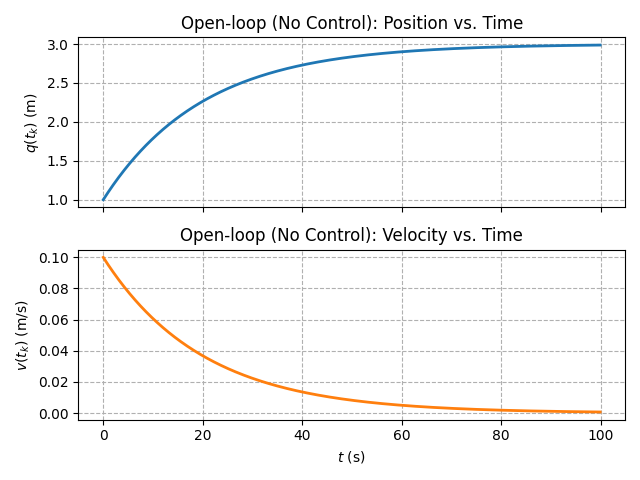
\includegraphics[width=0.85\linewidth]{Figure_1.png}
\caption{Open-loop response ($u_k=0$): $q_k$ and $v_k$ versus time.}
\end{figure}

\subsection*{(ii) With control ($u_k=-\mathbf{K}\mathbf{x}_k$)}

With the controller $u_k=-\mathbf{K}\mathbf{x}_k$, the update becomes
\[
\mathbf{x}_{k+1}=\bar{\mathbf{A}}\mathbf{x}_k,\qquad \bar{\mathbf{A}}=\mathbf{A}-\mathbf{B}\mathbf{K}.
\]
The eigenvalues of $\bar{\mathbf{A}}$ computed numerically are
\[
\mathrm{eig}(\bar{\mathbf{A}})=[0.90999965,\ 0.89000055]\quad \text{(from Python output)}.
\]
We again apply the criterion from part (c):
\[
\text{Stability requirement:}\quad |\mu_i|<1\ \ \forall i.
\]
For the provided $\mathbf{K}$, this condition is \emph{satisfied}. The plot shows both components decaying toward zero, matching the prediction that $\mathbf{x}_k\to\mathbf{0}$.

\begin{figure}[H]
\centering
\includegraphics[width=0.85\linewidth]{FIgure_2.png}
\caption{Closed-loop response ($u_k=-\mathbf{K}\mathbf{x}_k$): $q_k$ and $v_k$ versus time.}
\end{figure}

\end{document}